\documentclass[border=5pt,tikz]{standalone}
\usepackage{amsmath}
\usepackage{xcolor}
\usetikzlibrary{arrows.meta,positioning,fit,calc,shapes.multipart}

% Color palette (vivid)
\colorlet{cIntro}{teal!70!black}
\colorlet{cLR}{magenta!70!black}
\colorlet{cMeth}{orange!85!black}
\colorlet{cExp}{violet!85!black}
\colorlet{cDisc}{lime!60!black}
\colorlet{cAux}{cyan!70!black}

% Box styles
\tikzset{
  >={Latex[length=4.5pt,width=4.5pt]},
  box/.style={draw=#1, rounded corners=3pt, line width=0.9pt, fill=#1!10, align=left, inner sep=6pt, text width=8.8cm},
  subbox/.style={draw=#1, rounded corners=3pt, line width=0.8pt, fill=#1!12, align=left, inner sep=5pt, text width=6.8cm},
  sidebox/.style={draw=#1, rounded corners=3pt, line width=0.8pt, fill=#1!10, align=left, inner sep=5pt, text width=5.6cm},
  group/.style={draw=#1, dashed, rounded corners=4pt, line width=0.9pt, inner sep=8pt},
  title/.style={font=\bfseries},
  conn/.style={line width=1pt, #1},
}

\begin{document}
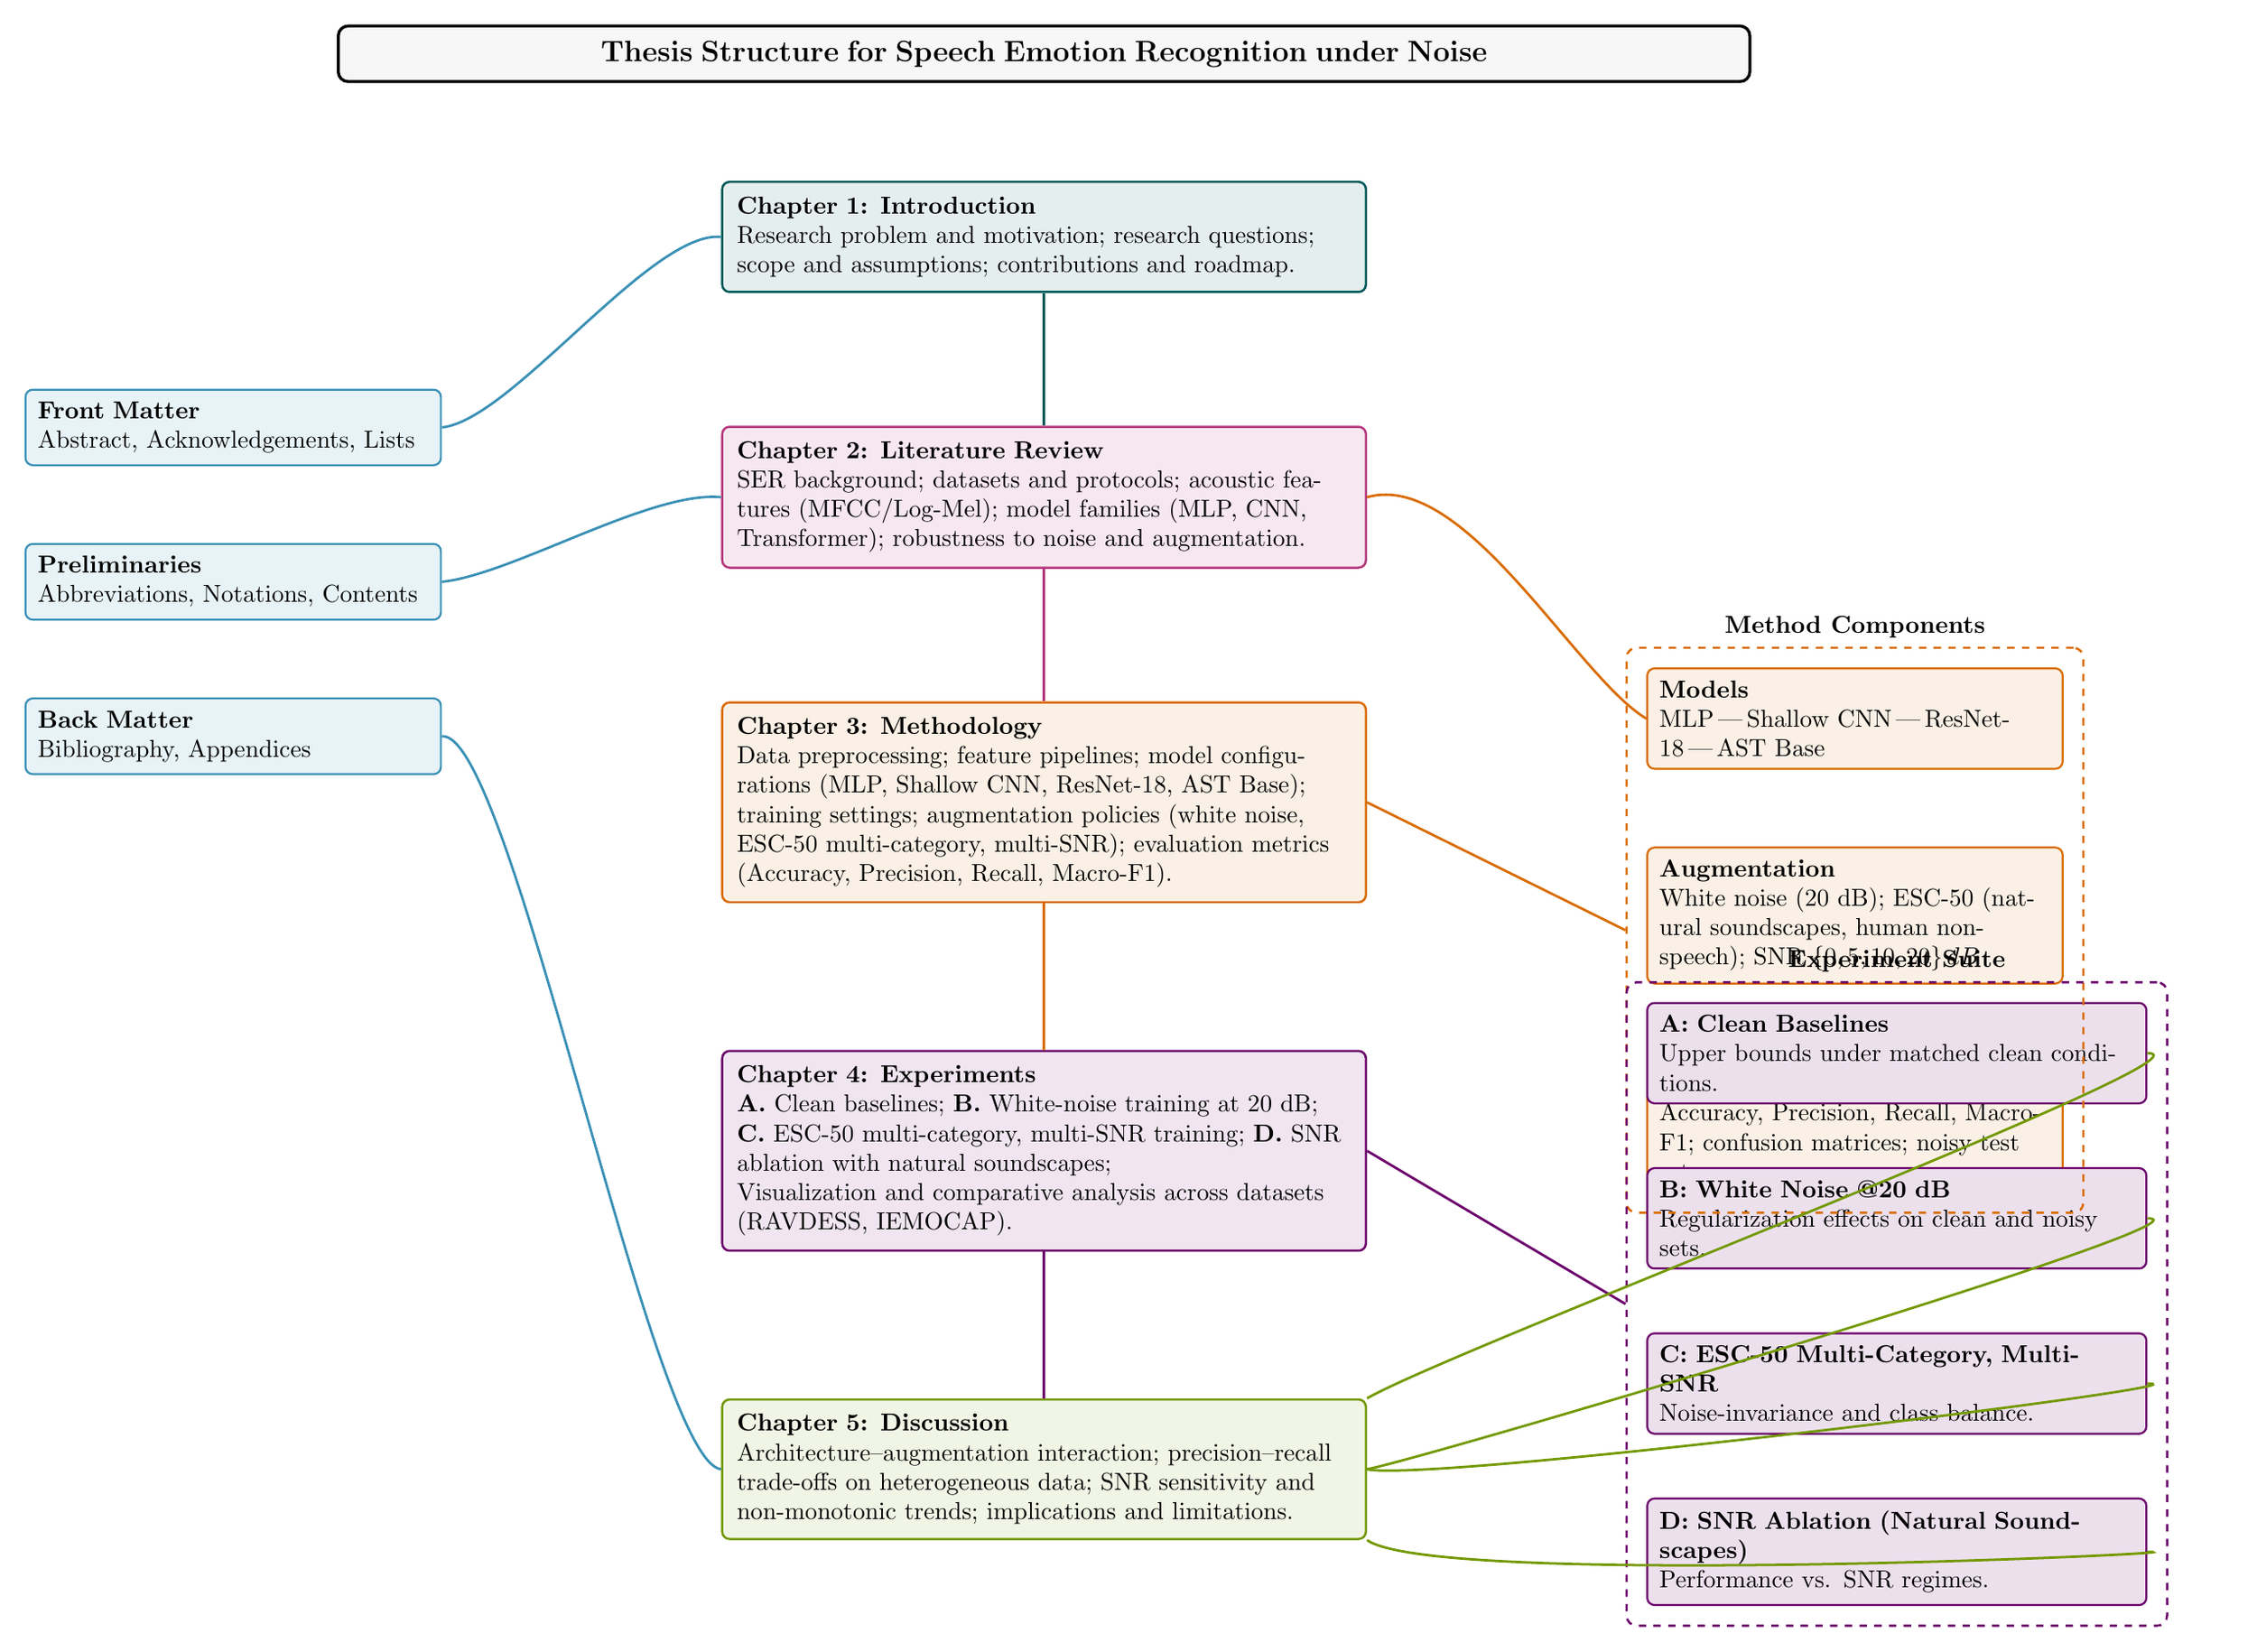
\begin{tikzpicture}[node distance=1.9cm and 1.6cm]

% Title
\node[draw=black, very thick, rounded corners=4pt, fill=black!3, align=center, inner sep=6pt, text width=19.8cm] (title)
  {\large\bfseries Thesis Structure for Speech Emotion Recognition under Noise};

% Central vertical flow: Chapters 1-5
\node[box=cIntro, below=1.4cm of title] (ch1) {\textbf{Chapter 1: Introduction}\\
Research problem and motivation; research questions; scope and assumptions; contributions and roadmap.};

\node[box=cLR, below=1.9cm of ch1] (ch2) {\textbf{Chapter 2: Literature Review}\\
SER background; datasets and protocols; acoustic features (MFCC/Log-Mel); model families (MLP, CNN, Transformer); robustness to noise and augmentation.};

\node[box=cMeth, below=1.9cm of ch2] (ch3) {\textbf{Chapter 3: Methodology}\\
Data preprocessing; feature pipelines; model configurations (MLP, Shallow CNN, ResNet-18, AST Base); training settings; augmentation policies (white noise, ESC-50 multi-category, multi-SNR); evaluation metrics (Accuracy, Precision, Recall, Macro-F1).};

\node[box=cExp, below=2.1cm of ch3] (ch4) {\textbf{Chapter 4: Experiments}\\
\textbf{A.} Clean baselines; \textbf{B.} White-noise training at 20 dB; \\
\textbf{C.} ESC-50 multi-category, multi-SNR training; \textbf{D.} SNR ablation with natural soundscapes;\\
Visualization and comparative analysis across datasets (RAVDESS, IEMOCAP).};

\node[box=cDisc, below=2.1cm of ch4] (ch5) {\textbf{Chapter 5: Discussion}\\
Architecture–augmentation interaction; precision–recall trade-offs on heterogeneous data; SNR sensitivity and non-monotonic trends; implications and limitations.};

% Side context blocks linked to Methodology / Experiments
\node[sidebox=cMeth, right=4.0cm of ch3, yshift=1.2cm] (models) {\textbf{Models}\\MLP\,|\,Shallow CNN\,|\,ResNet-18\,|\,AST Base};
\node[sidebox=cMeth, below=1.1cm of models] (aug) {\textbf{Augmentation}\\White noise (20 dB); ESC-50 (natural soundscapes, human non-speech); SNR \(\{0,5,10,20\}\,dB\)};
\node[sidebox=cMeth, below=1.1cm of aug] (metrics) {\textbf{Evaluation}\\Accuracy, Precision, Recall, Macro-F1; confusion matrices; noisy test sets.};

% Experiment sub-group on the right of Chapter 4
\node[subbox=cExp, right=4.0cm of ch4, yshift=1.4cm] (expA) {\textbf{A: Clean Baselines}\\Upper bounds under matched clean conditions.};
\node[subbox=cExp, below=0.9cm of expA] (expB) {\textbf{B: White Noise @20 dB}\\Regularization effects on clean and noisy sets.};
\node[subbox=cExp, below=0.9cm of expB] (expC) {\textbf{C: ESC-50 Multi-Category, Multi-SNR}\\Noise-invariance and class balance.};
\node[subbox=cExp, below=0.9cm of expC] (expD) {\textbf{D: SNR Ablation (Natural Soundscapes)}\\Performance vs. SNR regimes.};

% Fit groups (light dashed frames)
\node[group=cMeth, fit=(models)(aug)(metrics), label={[title]above:Method Components}] (gMeth) {};
\node[group=cExp, fit=(expA)(expB)(expC)(expD), label={[title]above:Experiment Suite}] (gExp) {};

% Inter-chapter arrows
\draw[conn=cIntro] (ch1) -- (ch2);
\draw[conn=cLR] (ch2) -- (ch3);
\draw[conn=cMeth] (ch3) -- (ch4);
\draw[conn=cExp] (ch4) -- (ch5);

% Cross links
\draw[conn=cMeth] (ch2.east) .. controls ($(ch2.east)+(1.4,0.4)$) and ($(models.west)+(-1.0,0.6)$) .. (models.west);
\draw[conn=cMeth] (ch3.east) -- (gMeth.west);
\draw[conn=cExp] (ch4.east) -- (gExp.west);
\draw[conn=cDisc] (expA.east) .. controls +(1.2,0) and +(1.2,0.7) .. (ch5.north east);
\draw[conn=cDisc] (expB.east) .. controls +(1.2,0) and +(1.0,0.2) .. (ch5.east);
\draw[conn=cDisc] (expC.east) .. controls +(1.2,0) and +(0.9,-0.2) .. (ch5.east);
\draw[conn=cDisc] (expD.east) .. controls +(1.2,0) and +(1.0,-0.7) .. (ch5.south east);

% Auxiliary flow (front/back matter)
\node[sidebox=cAux, left=4.0cm of ch2, yshift=1.0cm] (front) {\textbf{Front Matter}\\Abstract, Acknowledgements, Lists};
\node[sidebox=cAux, below=1.1cm of front] (pre) {\textbf{Preliminaries}\\Abbreviations, Notations, Contents};
\node[sidebox=cAux, below=1.1cm of pre] (biblio) {\textbf{Back Matter}\\Bibliography, Appendices};

\draw[conn=cAux] (front.east) .. controls +(1.0,0.1) and +(-1.0,0.1) .. (ch1.west);
\draw[conn=cAux] (pre.east) .. controls +(1.0,0.1) and +(-1.0,0.1) .. (ch2.west);
\draw[conn=cAux] (biblio.east) .. controls +(1.0,0.1) and +(-1.0,0.1) .. (ch5.west);

\end{tikzpicture}
\end{document}

